\documentclass[12pt,a4paper]{article}

\usepackage[a4paper,margin=1in]{geometry}
\usepackage[T1]{fontenc}
\usepackage[utf8]{inputenc}
\usepackage{tikz}
\usepackage{listings}
\usepackage{xcolor}
\usepackage{graphicx}
\usepackage{caption}

\lstset{
  basicstyle=\ttfamily\small,
  frame=single,
  breaklines=true,
  showstringspaces=false,
  columns=fullflexible
}

\begin{document}
\begin{titlepage}
    \centering
     \vspace*{2.5cm}
     {\LARGE \textbf{University of Chittagong}\par}
     {\Large Dept. of Computer Science \& Engineering \par}

    \vspace*{2cm}

    {\LARGE \textbf{DBMS Assignment}\par}
    \vspace{0.5cm}
    {\Large Tutorial-02 \par}
    Course Title: Database Management Systems\par
    Course Code: CSE-414\par
    \vspace{1.5cm}
     \textbf{Submitted to}\par
    \vspace{0.3cm}
    Course Instructor\par
    Dr.Rudra Pratap Deb Nath\par
    Professor\par
    Dept. of Computer Science \& engineering\par
    University of Chittagong\par
     \vspace{1.5cm}
    \textbf{Submitted by}\par
    \vspace{0.3cm}
    Team Name: ByteForge\par
    % ID: 24701009\par
    Department: Computer Science and Engineering\par
    Semester: 4th Semester\par

   

   
    

    \vfill

  
    

    \vspace{0.5cm}
    Submission Date:\par
    \today

\end{titlepage}
\setlength{\parindent}{0pt} % remove indentation globally
\setlength{\parskip}{6pt} 
\section*{Task:01}

\textbf{1.Document and describe your database in the way you would do it (or have done it) in a project report.}\par 


\textbf{Answer:}\par
\textbf{(I)Introduction:}
This database is designed to store and manage medical information related to drugs,disease and their relationships.The system is designed to support queries that analyze drug–disease relationships, identify common side effects, and explore clinical trial data efficiently so that users can retrieve meaningful insights about drugs and their applications.\par
\textbf{(II)Scoop of the Database:}
The database includes the following types of information:\par
1.Drugs and their categories.\par
2.Diseases and their categories.\par
3.Side effects and Interactions of Drugs.\par
4.Commercial Drug Products and Companies.\par
5.Clinical trial information and their researcher and location.\par
\textbf{(III)Assumption:}
To simplify the design, the following assumptions are made:\par
1.A drug can treat multiple diseases.\par
2.A disease can be treated by multiple drugs.\par
3.A drug can have multiple side effects.\par
4.A side effect can be caused by multiple drugs.\par
5.Drug interactions occur between two or more drugs.\par
6.A drug may have multiple commercial products.\par
7.A drug may be involved in multiple clinical trials.\par
\textbf{(IV)Entities \& Relationship}\par
\textbf{Entities:}\par
1.Drug\par
2.Disease\par
3.Side-effect\par
4.Clinical Trial\par
5.Researcher\par
6.product\par
7.Company\par
\textbf{Relationship:}\par
1.Drugs and Diseases(M:N)\par
2.Drugs and Side Effects(1:N)\par
3.Drugs and Clinical Trials(M:N)\par
4.Drugs can interact with other Drugs (self-relationship)\par
5.Drugs and Products(1:N)\par
6.Products and company(N:1)\par
7.Clinical trials and Researcher(1:1)\par



\textbf{2. Provide a list of tables with attributes that you would use to store your data.}\par

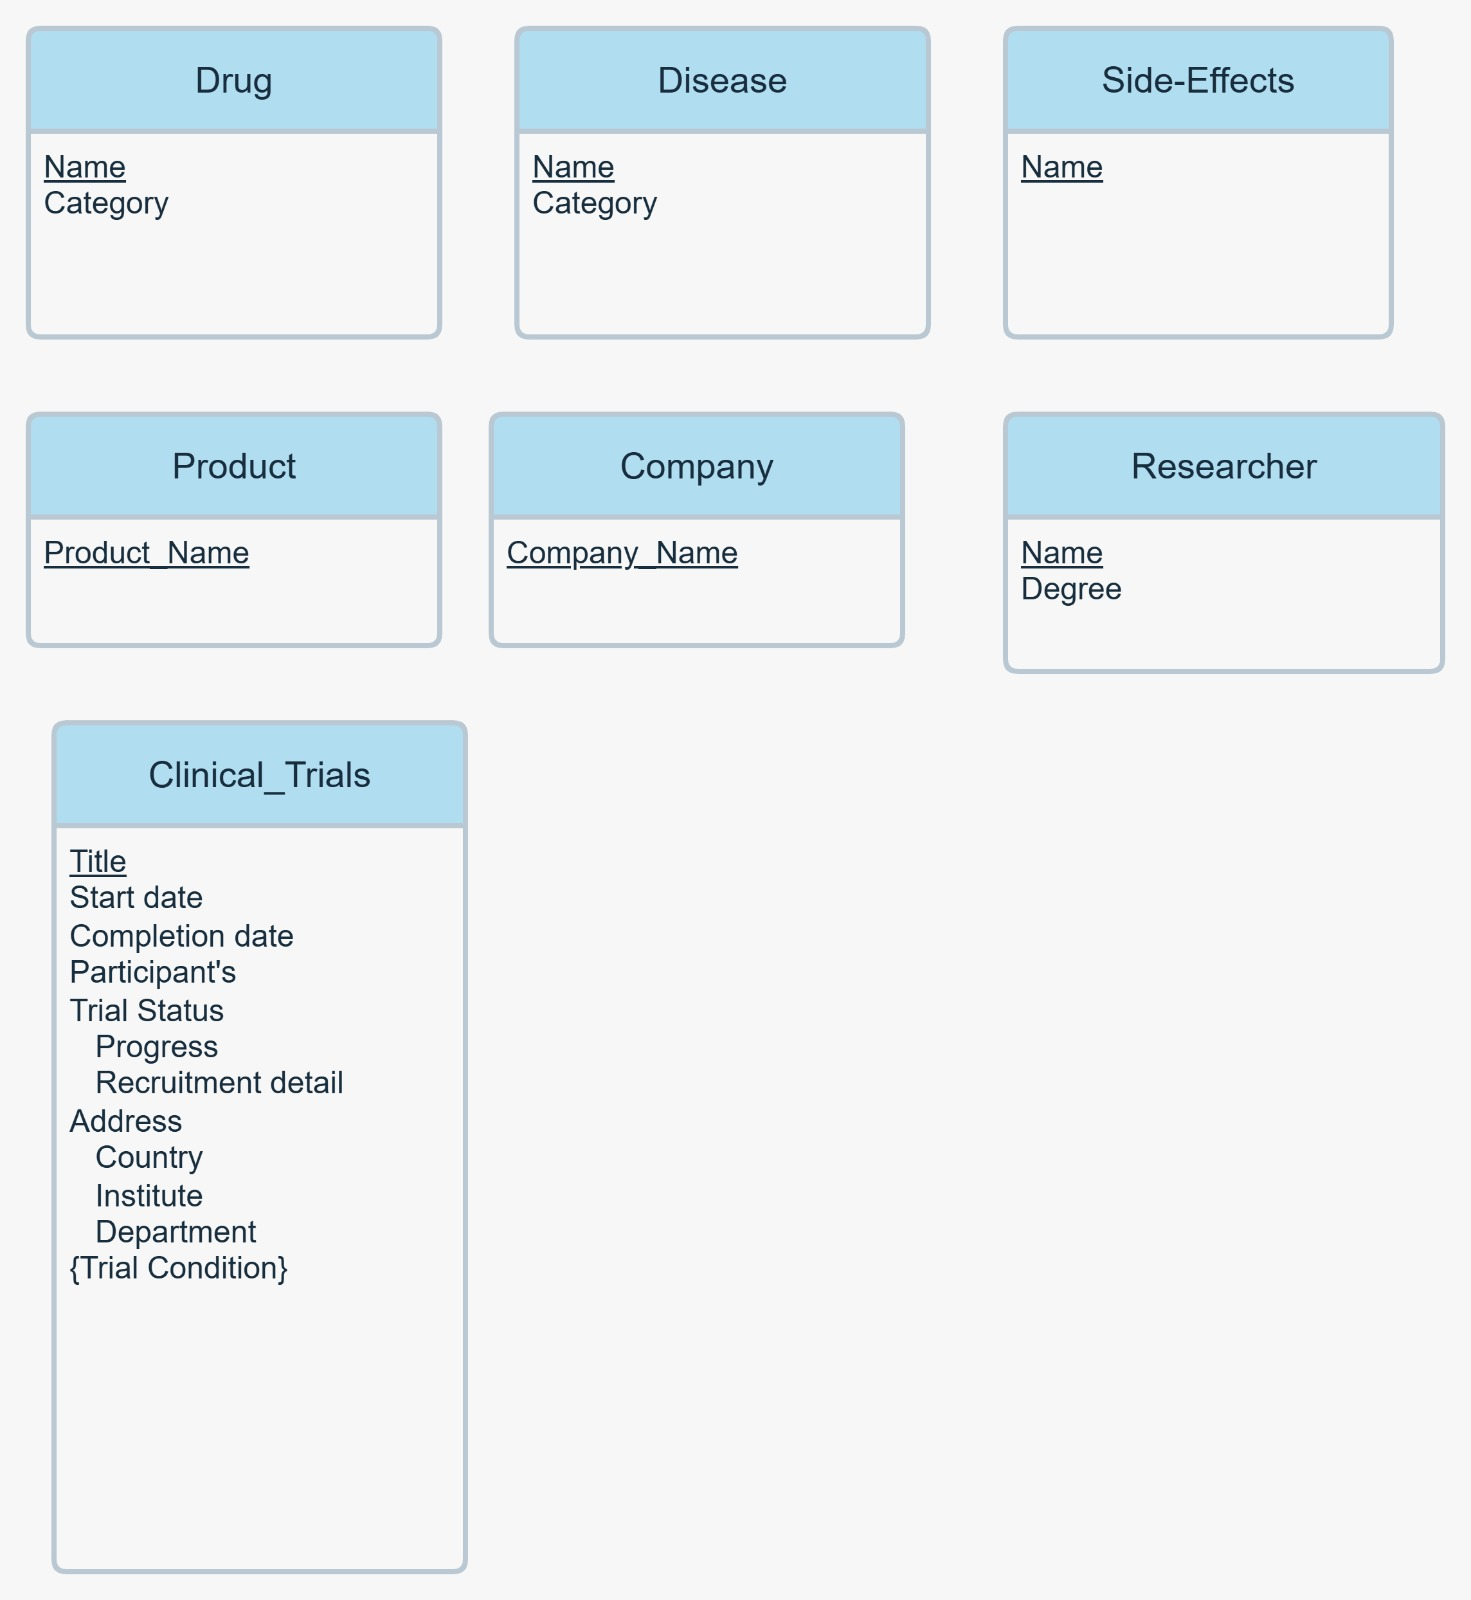
\includegraphics[width=0.8\textwidth]{Task1.jpeg}\par
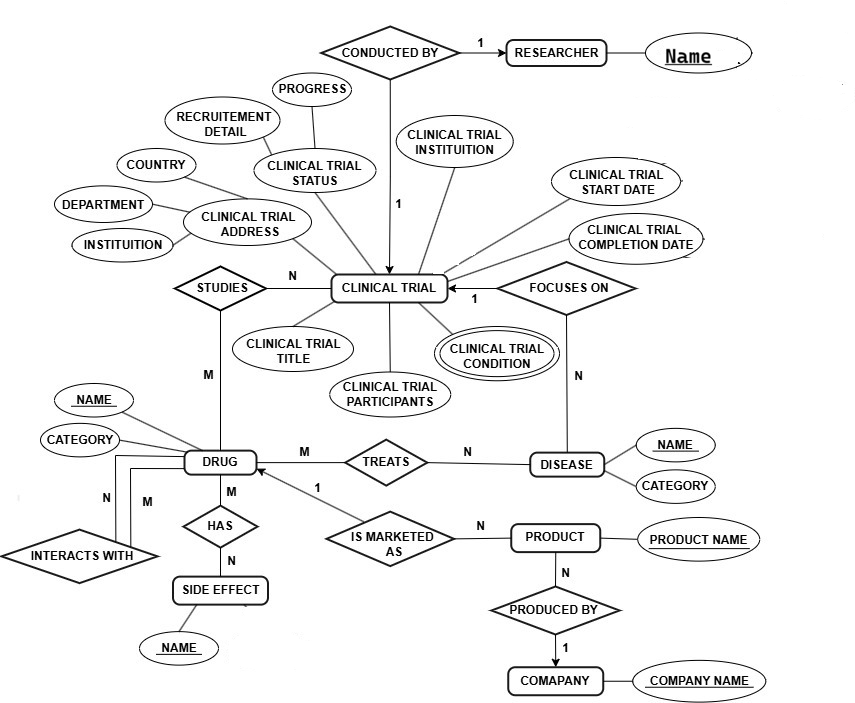
\includegraphics[width=0.8\textwidth]{Final1.png}\par


\newpage
\textbf{3. In case you already have a good command of SQL, add the SQL commands that create your database.}\par

\textbf{Answer:}\par

\textbf{DATABASE}\par
\begin{lstlisting}[language=SQL,breaklines=true]
DROP DATABASE IF EXISTS PHARMA_DB;
CREATE DATABASE IF NOT EXISTS PHARMA_DB;
USE PHARMA_DB;

-- =========================
-- MAIN ENTITY TABLES
-- =========================

CREATE TABLE IF NOT EXISTS DRUG (
    DRUG_NAME       VARCHAR(255) PRIMARY KEY,
    DRUG_CATEGORY   VARCHAR(255)
);

CREATE TABLE IF NOT EXISTS DISEASE (
    DISEASE_NAME       VARCHAR(255) PRIMARY KEY,
    DISEASE_CATEGORY   VARCHAR(255)
);

CREATE TABLE IF NOT EXISTS SIDE_EFFECT (
    SIDE_EFFECT_NAME   VARCHAR(255) PRIMARY KEY
);

CREATE TABLE IF NOT EXISTS RESEARCHER (
    MAIN_RESEARCHER    VARCHAR(255) PRIMARY KEY
);

CREATE TABLE IF NOT EXISTS COMPANY (
    COMPANY_NAME       VARCHAR(255) PRIMARY KEY
);

CREATE TABLE IF NOT EXISTS PRODUCT (
    PRODUCT_NAME       VARCHAR(255) PRIMARY KEY
);

CREATE TABLE IF NOT EXISTS CLINICAL_TRIAL (
    CLINICAL_TRIAL_TITLE             VARCHAR(500) PRIMARY KEY,
    CLINICAL_TRIAL_STATUS            VARCHAR(100),
    CLINICAL_TRIAL_COUNTRY           VARCHAR(255),
    CLINICAL_TRIAL_DEPARTMENT        VARCHAR(255),
    CLINICAL_TRIAL_INSTITUTION       VARCHAR(255),
    CLINICAL_TRIAL_START_DATE        DATE,
    CLINICAL_TRIAL_COMPLETION_DATE   DATE,
    CLINICAL_TRIAL_CONDITION         VARCHAR(255),
    CLINICAL_TRIAL_PARTICIPANTS      INT
);

-- =========================
-- RELATIONSHIP TABLES
-- =========================
CREATE TABLE IF NOT EXISTS STUDIES (
    CLINICAL_TRIAL_TITLE   VARCHAR(500),
    DRUG_NAME              VARCHAR(255),
    PRIMARY KEY (CLINICAL_TRIAL_TITLE, DRUG_NAME),
    CONSTRAINT FK_STUDIES_TRIAL FOREIGN KEY (CLINICAL_TRIAL_TITLE)
        REFERENCES CLINICAL_TRIAL(CLINICAL_TRIAL_TITLE)
        ON DELETE CASCADE
        ON UPDATE CASCADE,
    CONSTRAINT FK_STUDIES_DRUG FOREIGN KEY (DRUG_NAME)
        REFERENCES DRUG(DRUG_NAME)
        ON DELETE CASCADE
        ON UPDATE CASCADE
);
-- TREATS : DRUG (M) <-> (N) DISEASE
CREATE TABLE IF NOT EXISTS TREATS (
    DRUG_NAME        VARCHAR(255),
    DISEASE_NAME     VARCHAR(255),
    PRIMARY KEY (DRUG_NAME, DISEASE_NAME),
    CONSTRAINT FK_TREATS_DRUG FOREIGN KEY (DRUG_NAME)
        REFERENCES DRUG(DRUG_NAME)
        ON DELETE CASCADE
        ON UPDATE CASCADE,
    CONSTRAINT FK_TREATS_DISEASE FOREIGN KEY (DISEASE_NAME)
        REFERENCES DISEASE(DISEASE_NAME)
        ON DELETE CASCADE
        ON UPDATE CASCADE
);
-- HAS : DRUG (M) <-> (N) SIDE_EFFECT
CREATE TABLE IF NOT EXISTS HAS_SIDE_EFFECT (
    DRUG_NAME          VARCHAR(255),
    SIDE_EFFECT_NAME   VARCHAR(255),
    PRIMARY KEY (DRUG_NAME, SIDE_EFFECT_NAME),
    CONSTRAINT FK_HAS_DRUG FOREIGN KEY (DRUG_NAME)
        REFERENCES DRUG(DRUG_NAME)
        ON DELETE CASCADE
        ON UPDATE CASCADE,
    CONSTRAINT FK_HAS_SIDE_EFFECT FOREIGN KEY (SIDE_EFFECT_NAME)
        REFERENCES SIDE_EFFECT(SIDE_EFFECT_NAME)
        ON DELETE CASCADE
        ON UPDATE CASCADE
);
-- INTERACTS_WITH : recursive M:N on DRUG
CREATE TABLE IF NOT EXISTS INTERACTS_WITH (
    DRUG_NAME                 VARCHAR(255),
    INTERACTS_WITH_DRUG_NAME  VARCHAR(255),
    PRIMARY KEY (DRUG_NAME, INTERACTS_WITH_DRUG_NAME),
    CONSTRAINT FK_INTERACTS_DRUG1 FOREIGN KEY (DRUG_NAME)
        REFERENCES DRUG(DRUG_NAME)
        ON DELETE CASCADE
        ON UPDATE CASCADE,
    CONSTRAINT FK_INTERACTS_DRUG2 FOREIGN KEY (INTERACTS_WITH_DRUG_NAME)
        REFERENCES DRUG(DRUG_NAME)
        ON DELETE CASCADE
        ON UPDATE CASCADE
);
-- CONDUCTED_BY : CLINICAL_TRIAL (1) <-> (1) RESEARCHER
CREATE TABLE IF NOT EXISTS CONDUCTED_BY (
    CLINICAL_TRIAL_TITLE   VARCHAR(500) PRIMARY KEY,
    MAIN_RESEARCHER        VARCHAR(255) UNIQUE,
    CONSTRAINT FK_CB_TRIAL FOREIGN KEY (CLINICAL_TRIAL_TITLE)
        REFERENCES CLINICAL_TRIAL(CLINICAL_TRIAL_TITLE)
        ON DELETE CASCADE
        ON UPDATE CASCADE,
    CONSTRAINT FK_CB_RESEARCHER FOREIGN KEY (MAIN_RESEARCHER)
        REFERENCES RESEARCHER(MAIN_RESEARCHER)
        ON DELETE CASCADE
        ON UPDATE CASCADE
);
-- FOCUSES_ON : CLINICAL_TRIAL (1) -> (N) DISEASE
-- One clinical trial focuses on one disease entry here
-- A disease can appear in many trials
CREATE TABLE IF NOT EXISTS FOCUSES_ON (
    CLINICAL_TRIAL_TITLE   VARCHAR(500) PRIMARY KEY,
    DISEASE_NAME           VARCHAR(255),
    CONSTRAINT FK_FO_TRIAL FOREIGN KEY (CLINICAL_TRIAL_TITLE)
        REFERENCES CLINICAL_TRIAL(CLINICAL_TRIAL_TITLE)
        ON DELETE CASCADE
        ON UPDATE CASCADE,
    CONSTRAINT FK_FO_DISEASE FOREIGN KEY (DISEASE_NAME)
        REFERENCES DISEASE(DISEASE_NAME)
        ON DELETE CASCADE
        ON UPDATE CASCADE
);
-- IS_MARKETED_AS : DRUG (1) -> (N) PRODUCT
-- One drug can have many products
-- Each product belongs to one drug
CREATE TABLE IF NOT EXISTS IS_MARKETED_AS (
    PRODUCT_NAME      VARCHAR(255) PRIMARY KEY,
    DRUG_NAME         VARCHAR(255),
    CONSTRAINT FK_IMA_PRODUCT FOREIGN KEY (PRODUCT_NAME)
        REFERENCES PRODUCT(PRODUCT_NAME)
        ON DELETE CASCADE
        ON UPDATE CASCADE,
    CONSTRAINT FK_IMA_DRUG FOREIGN KEY (DRUG_NAME)
        REFERENCES DRUG(DRUG_NAME)
        ON DELETE CASCADE
        ON UPDATE CASCADE
);
-- PRODUCED_BY : PRODUCT (N) -> (1) COMPANY
CREATE TABLE IF NOT EXISTS PRODUCED_BY (
    PRODUCT_NAME      VARCHAR(255) PRIMARY KEY,
    COMPANY_NAME      VARCHAR(255),
    CONSTRAINT FK_PB_PRODUCT FOREIGN KEY (PRODUCT_NAME)
        REFERENCES PRODUCT(PRODUCT_NAME)
        ON DELETE CASCADE
        ON UPDATE CASCADE,
    CONSTRAINT FK_PB_COMPANY FOREIGN KEY (COMPANY_NAME)
        REFERENCES COMPANY(COMPANY_NAME)
        ON DELETE CASCADE
        ON UPDATE CASCADE
);

\end{lstlisting}
\newpage
\textbf{Python SCRIPT}\par
\begin{lstlisting}[language=Python,breaklines=true]
import pandas as pd
import os
import mysql.connector
from mysql.connector import Error
from collections import defaultdict

# ========== CONFIGURATION ==========
# EXCEL_FILE = "sample.xlsx"
BASE_DIR = os.path.dirname(os.path.abspath(__file__))
EXCEL_FILE = os.path.join(BASE_DIR, "sample.xlsx")
DB_CONFIG = {
    "host": "localhost",
    "user": "sheikh",          # change as needed
    "password": "miniso123",          # set your MySQL root password
    "database": "PHARMA_DB_TASK1"
}

# ========== HELPER FUNCTIONS ==========
def clean_str(val):
    """Convert to string, strip, return None if empty or NaN."""
    if pd.isna(val):
        return None
    s = str(val).strip()
    return s if s else None

def get_side_effects(row):
    """Extract non-empty side effects from columns B-F (indices 1-5)."""
    effects = []
    for i in range(1, 6):  # columns B to F
        eff = clean_str(row.iloc[i])
        if eff:
            effects.append(eff)
    return effects

def get_interacts(row):
    """Extract non-empty interacting drugs from columns G-I (indices 6-8)."""
    interacts = []
    for i in range(6, 9):
        drug = clean_str(row.iloc[i])
        if drug:
            interacts.append(drug)
    return interacts

# ========== MAIN IMPORT ==========
def main():
    # 1. Read Excel
    df = pd.read_excel(EXCEL_FILE, sheet_name="Sheet1", header=0)
    # Rename columns for easier access (optional)
    # Expected columns order:
    # 0:A drug_name, 1:B side_effect1, 2:C side_effect2, 3:D side_effect3, 4:E side_effect4, 5:F side_effect5,
    # 6:G interacts1, 7:H interacts2, 8:I interacts3, 9:J disease_name, 10:K disease_category,
    # 11:L drug_category, 12:M product_name, 13:N company_name, 14:O clinical_trial_title,
    # 15:P start_date, 16:Q completion_date, 17:R participants, 18:S status,
    # 19:T condition1, 20:U condition2, 21:V address/country, 22:W institution,
    # 23:X department, 24:Y main_researcher, 25:Z condition3
    # We'll use iloc positions.

    # Data containers
    drugs = {}                # drug_name -> set of categories
    diseases = {}             # disease_name -> disease_category
    side_effects = set()
    researchers = set()
    companies = set()
    products = {}             # product_name -> (drug_name, company_name)
    clinical_trials = {}      # trial_title -> dict of attributes
    interacts_set = set()     # (drug_name, interacts_with)
    treats_set = set()        # (drug_name, disease_name)
    has_side_effect_set = set()  # (drug_name, side_effect)
    studies_set = set()       # (trial_title, drug_name)
    conducted_by_dict = {}    # trial_title -> researcher
    focuses_on_dict = {}      # trial_title -> disease_name (first condition)
    is_marketed_as_dict = {}  # product_name -> drug_name
    produced_by_dict = {}     # product_name -> company_name

    # 2. Iterate rows
    for idx, row in df.iterrows():
        drug_name = clean_str(row.iloc[0])
        if not drug_name:
            # Skip rows without a drug name (they are incomplete/duplicate entries)
            continue

        # --- Drug & Category ---
        drug_cat = clean_str(row.iloc[11])
        if drug_cat:
            if drug_name not in drugs:
                drugs[drug_name] = set()
            drugs[drug_name].add(drug_cat)

        # --- Disease & Category ---
        disease_name = clean_str(row.iloc[9])
        disease_cat = clean_str(row.iloc[10])
        if disease_name:
            diseases[disease_name] = disease_cat
            # Treats relationship
            treats_set.add((drug_name, disease_name))

        # --- Side Effects ---
        for effect in get_side_effects(row):
            side_effects.add(effect)
            has_side_effect_set.add((drug_name, effect))

        # --- Interacts With ---
        for interact_drug in get_interacts(row):
            # Ensure the interacting drug exists in drugs set (will be added later)
            # We will add it to drugs with unknown category later.
            if interact_drug not in drugs:
                drugs[interact_drug] = set()  # placeholder, category unknown
            interacts_set.add((drug_name, interact_drug))

        # --- Product & Company ---
        product_name = clean_str(row.iloc[12])
        company_name = clean_str(row.iloc[13])
        if product_name and company_name:
            products[product_name] = (drug_name, company_name)
            is_marketed_as_dict[product_name] = drug_name
            produced_by_dict[product_name] = company_name
            companies.add(company_name)

        # --- Clinical Trial ---
        trial_title = clean_str(row.iloc[14])
        if trial_title:
            # Check if we already processed this trial
            if trial_title not in clinical_trials:
                # Extract trial attributes
                start = row.iloc[15]
                completion = row.iloc[16]
                participants = row.iloc[17]
                status = clean_str(row.iloc[18])
                country = clean_str(row.iloc[21])   # column V
                institution = clean_str(row.iloc[22]) # column W
                department = clean_str(row.iloc[23])  # column X
                # Convert dates
                start_date = pd.to_datetime(start).date() if pd.notna(start) else None
                end_date = pd.to_datetime(completion).date() if pd.notna(completion) else None
                participants_int = int(participants) if pd.notna(participants) else None
                # First condition (column T) for FOCUSES_ON
                condition1 = clean_str(row.iloc[19])
                clinical_trials[trial_title] = {
                    "status": status,
                    "country": country,
                    "department": department,
                    "institution": institution,
                    "start_date": start_date,
                    "completion_date": end_date,
                    "condition": condition1,   # for focus
                    "participants": participants_int
                }
            else:
                # If trial already exists, maybe update condition? Use first encountered.
                pass

            # Studies relationship
            studies_set.add((trial_title, drug_name))

            # Conducted By (researcher)
            researcher = clean_str(row.iloc[24])
            if researcher:
                researchers.add(researcher)
                conducted_by_dict[trial_title] = researcher

            # Focuses On (use condition from column T, only if not already set)
            # Use the first condition we see; if already set, keep original.
            if trial_title not in focuses_on_dict:
                cond = clean_str(row.iloc[19])
                if cond:
                    focuses_on_dict[trial_title] = cond

    # 3. Insert into MySQL
    try:
        conn = mysql.connector.connect(**DB_CONFIG)
        cursor = conn.cursor()
        # Disable foreign key checks for bulk insert order
        cursor.execute("SET FOREIGN_KEY_CHECKS = 0")

        # ---- Insert DRUGS (with concatenated categories) ----
        for drug_name, cat_set in drugs.items():
            cat_str = ", ".join(sorted(cat_set)) if cat_set else None
            cursor.execute(
                "INSERT IGNORE INTO DRUG (DRUG_NAME, DRUG_CATEGORY) VALUES (%s, %s)",
                (drug_name, cat_str)
            )

        # ---- Insert DISEASE ----
        for disease_name, disease_cat in diseases.items():
            cursor.execute(
                "INSERT IGNORE INTO DISEASE (DISEASE_NAME, DISEASE_CATEGORY) VALUES (%s, %s)",
                (disease_name, disease_cat)
            )

        # ---- Insert SIDE_EFFECT ----
        for effect in side_effects:
            cursor.execute(
                "INSERT IGNORE INTO SIDE_EFFECT (SIDE_EFFECT_NAME) VALUES (%s)",
                (effect,)
            )

        # ---- Insert RESEARCHER ----
        for researcher in researchers:
            cursor.execute(
                "INSERT IGNORE INTO RESEARCHER (MAIN_RESEARCHER) VALUES (%s)",
                (researcher,)
            )

        # ---- Insert COMPANY ----
        for company in companies:
            cursor.execute(
                "INSERT IGNORE INTO COMPANY (COMPANY_NAME) VALUES (%s)",
                (company,)
            )

        # ---- Insert PRODUCT ----
        for product_name in products.keys():
            cursor.execute(
                "INSERT IGNORE INTO PRODUCT (PRODUCT_NAME) VALUES (%s)",
                (product_name,)
            )

        # ---- Insert CLINICAL_TRIAL ----
        for title, attrs in clinical_trials.items():
            cursor.execute("""
                INSERT IGNORE INTO CLINICAL_TRIAL (
                    CLINICAL_TRIAL_TITLE, CLINICAL_TRIAL_STATUS, CLINICAL_TRIAL_COUNTRY,
                    CLINICAL_TRIAL_DEPARTMENT, CLINICAL_TRIAL_INSTITUTION,
                    CLINICAL_TRIAL_START_DATE, CLINICAL_TRIAL_COMPLETION_DATE,
                    CLINICAL_TRIAL_CONDITION, CLINICAL_TRIAL_PARTICIPANTS
                ) VALUES (%s, %s, %s, %s, %s, %s, %s, %s, %s)
            """, (
                title, attrs["status"], attrs["country"],
                attrs["department"], attrs["institution"],
                attrs["start_date"], attrs["completion_date"],
                attrs["condition"], attrs["participants"]
            ))

        # ---- Relationship tables ----
        # TREATS
        for drug_name, disease_name in treats_set:
            cursor.execute(
                "INSERT IGNORE INTO TREATS (DRUG_NAME, DISEASE_NAME) VALUES (%s, %s)",
                (drug_name, disease_name)
            )

        # HAS_SIDE_EFFECT
        for drug_name, effect in has_side_effect_set:
            cursor.execute(
                "INSERT IGNORE INTO HAS_SIDE_EFFECT (DRUG_NAME, SIDE_EFFECT_NAME) VALUES (%s, %s)",
                (drug_name, effect)
            )

        # INTERACTS_WITH
        for drug_name, interact_drug in interacts_set:
            cursor.execute(
                "INSERT IGNORE INTO INTERACTS_WITH (DRUG_NAME, INTERACTS_WITH_DRUG_NAME) VALUES (%s, %s)",
                (drug_name, interact_drug)
            )

        # STUDIES
        for trial_title, drug_name in studies_set:
            cursor.execute(
                "INSERT IGNORE INTO STUDIES (CLINICAL_TRIAL_TITLE, DRUG_NAME) VALUES (%s, %s)",
                (trial_title, drug_name)
            )

        # CONDUCTED_BY
        for trial_title, researcher in conducted_by_dict.items():
            cursor.execute(
                "INSERT IGNORE INTO CONDUCTED_BY (CLINICAL_TRIAL_TITLE, MAIN_RESEARCHER) VALUES (%s, %s)",
                (trial_title, researcher)
            )

        # FOCUSES_ON
        for trial_title, disease_name in focuses_on_dict.items():
            cursor.execute(
                "INSERT IGNORE INTO FOCUSES_ON (CLINICAL_TRIAL_TITLE, DISEASE_NAME) VALUES (%s, %s)",
                (trial_title, disease_name)
            )

        # IS_MARKETED_AS
        for product_name, drug_name in is_marketed_as_dict.items():
            cursor.execute(
                "INSERT IGNORE INTO IS_MARKETED_AS (PRODUCT_NAME, DRUG_NAME) VALUES (%s, %s)",
                (product_name, drug_name)
            )

        # PRODUCED_BY
        for product_name, company_name in produced_by_dict.items():
            cursor.execute(
                "INSERT IGNORE INTO PRODUCED_BY (PRODUCT_NAME, COMPANY_NAME) VALUES (%s, %s)",
                (product_name, company_name)
            )

        # Re-enable foreign key checks
        cursor.execute("SET FOREIGN_KEY_CHECKS = 1")
        conn.commit()
        print("Data imported successfully!")

    except Error as e:
        print(f"Error: {e}")
        conn.rollback()
    finally:
        if conn.is_connected():
            cursor.close()
            conn.close()

if __name__ == "__main__":
    main()
\end{lstlisting}

\newpage
\section*{Task:02}
\textbf{1. Identify relevant data (consider the sample queries included in this document).}\par
\textbf{Answer}\par
To design the database, the relevant data is identified based on the requirements and sample queries. The goal is to determine what information must be stored so that all required queries can be answered efficiently.\par
$\rightarrow$ Identified Data Entities and Attributes\par
1.Drug\par
drug\_name(PK)\par
drug\_category\par
interacts\_with\par
*Needed for:
almost all queries (a, b, c, d, e, f, g, h, i)\par
2.Side Effect\par
side\_effect\_name(PK)\par

*Needed for:\par

(a) nausea\par
(c) cough and headache\par
(g) top side effects\par
3.Disease\par
disease\_name(PK)\par
disease\_category\par
Needed for:\par
(d) endocrine diseases\par
(e) immunological vs hematological\par
(f) hydrocortisone vs etanercept\par
(j, k) respiratory \& cardiovascular\par
4.Product\par
product\_name(PK)\par
company\_name\par
5.Clinical Trial\par
title(PK)\par
status\par
start\_date\par
-Needed for query (i)\par
completion\_date\par
-Needed for query (i)\par
participants\par
-Needed for query (h) \par
condition\par
address(Composite attribute: country, department, institution)\par 
-Needed for query (l)\par
6.Researcher\par
Name(PK)\par
\begin{table}[h]
\centering
\renewcommand{\arraystretch}{1.4}
\begin{tabular}{|l|l|l|l|}
\hline
\textbf{Relationship} & \textbf{Entities Involved} & \textbf{Cardinality} & \textbf{Queries Supported} \\
\hline
treats & Drug $\leftrightarrow$ Disease & M:N & (d), (e), (f), (g) \\
\hline
has & Drug $\leftrightarrow$ Side Effect & M:N & (a), (c), (g) \\
\hline
is marketed as & Drug $\rightarrow$ Product & 1:N & commercial product lookup \\
\hline
interacts with & Drug $\leftrightarrow$ Drug & M:N (self-ref) & (b) \\
\hline
studies & Clinical Trial $\leftrightarrow$ Drug & M:N & (h), (i), (j), (k) \\
\hline
conducted by & Clinical Trial $\rightarrow$ Researcher & N:1 & (j), (k) \\
\hline
\end{tabular}

\label{tab:relationships}
\end{table}
\end{document}
